% Autor: Pablo Baeyens (@pbaeyens)
% Email: pbaeyens31+github@gmail.com
% Licencia: CC BY-SA 3.0

%% Paquetes y configuración %

% Beamer
\PassOptionsToPackage{unicode}{hyperref}  % Evita errores con caracteres no ASCII
\PassOptionsToPackage{naturalnames}{hyperref} % tex.stackexchange.com/questions/10555
\documentclass[compress]{beamer}

% Idioma
\usepackage[spanish]{babel} % Traducciones
\usepackage[utf8]{inputenc} % Uso de caracteres UTF-8
\usepackage{lmodern}        % Fuentes de tamaño arbitrario
\usepackage[T1]{fontenc}    % Permite copiar y evita errores
\uselanguage{Spanish}       % Traducciones beamer
\languagepath{Spanish}      % (tex.stackexchange.com/questions/168208)

% Matemáticas
\usepackage{amsfonts}
\usepackage{amsmath}
\usepackage{amssymb}
\usepackage{marginnote}
% Colores
\definecolor{backg}{HTML}{F2F2F2}    % Fondo
\definecolor{title}{HTML}{bdc3d1}    % Títulos
\definecolor{comments}{HTML}{BDBDBD} % Comentarios
\definecolor{keywords}{HTML}{08388c} % Palabras clave
\definecolor{strings}{HTML}{FA5858}  % Strings
\definecolor{links}{HTML}{2C2C95}    % Enlaces
\definecolor{bars}{HTML}{045FB4}     % Barras (gráfico)

% Código
\usepackage{listings}
\lstset{
language=[LaTeX]TeX,
basicstyle=\footnotesize,
morekeywords={href,uselanguage,languagepath,column},
otherkeywords={pause,usetheme,usecolortheme,useinnertheme,titlepage,tableofcontents,subtitle},
breaklines=true,
backgroundcolor=\color{backg},
keywordstyle=\color{keywords},
commentstyle=\color{comments},
stringstyle=\color{strings},
tabsize=2,
% Acentos, ñ, ¿, ¡ (tex.stackexchange.com/questions/24528)
extendedchars=true,
literate={á}{{\'a}}1 {é}{{\'e}}1 {í}{{\'i}}1 {ó}{{\'o}}1
         {ú}{{\'u}}1 {ñ}{{\~n}}1 {¡}{{\textexclamdown}}1
         {¿}{{?`}}1
}

% Gráficos
\usepackage{pgfplots}
\pgfplotsset{width=7cm,compat=1.8} % Opciones para gráficos

% Emoticonos
\usepackage{wasysym}
\usepackage{graphicx}
% tikz
\usepackage{tikz}
\usetikzlibrary{mindmap,trees,shadows}
\tikzset{ % Genera overlays
    invisible/.style={opacity=0},
    visible on/.style={alt={#1{}{invisible}}},
    alt/.code args={<#1>#2#3}{\alt<#1>{\pgfkeysalso{#2}}{\pgfkeysalso{#3}}},
}

%% Comandos %%
\newcommand{\ejemplo}[1]{\lstinputlisting{./examples/#1}} % Mostrar código de ejemplos
\newcommand{\muestra}[1]{\input{./examples/#1}}           % Mostrar ejemplos
\newcommand{\seccion}[1]{\input{./sections/#1}}           % Incluir secciones
\newcommand{\espacio}{\vspace*{\baselineskip}}            % Añade espacios
\newcommand{\beamer}{\texttt{beamer} }                    % Estilo único para beamer
\newcommand{\enlace}[3]{\href{#1}{\textbf{#2}} - {\small #3}}  % Estílo único para refs
\newcommand{\comando}[1]{{\color{black}\textbackslash}{\color{keywords}#1}}
\newcommand{\marginalnote}[1]{\mbox{}\marginpar{\raggedright\hspace{0pt}#1}}
%% Temas %%
% Tema y tema de color
  \usetheme{Dresden}
  \usecolortheme{dolphin}
  \useinnertheme{circles}
  \setbeamercovered{transparent}
% Colores bloques
  \setbeamercolor{block title}{bg=title,fg=links}
  \setbeamercolor{block body}{bg=backg,fg=black}
  \setbeamercolor{block title alerted}{fg=red!70!black,bg=title!92!red}
  \setbeamercolor{block body alerted}{fg=black,bg=backg}
  \setbeamercolor{block title example}{fg=green!70!black,bg=title!92!green}
  \setbeamercolor{block body example}{fg=black,bg=backg}
% Enlaces (tex.stackexchange.com/questions/13423)
\hypersetup{colorlinks,linkcolor=,urlcolor=links}
% Quita enlaces de navegación (stackoverflow.com/questions/3017030)
\setbeamertemplate{navigation symbols}{}
% Quita barra inferior (stackoverflow.com/questions/1435837)
\setbeamertemplate{footline}{}
% Evita warnings boxes
\hfuzz=20pt
\vfuzz=20pt
% Evita wranings itemize
\renewcommand\textbullet{\ensuremath{\bullet}}

%% Título y otros %%
\title{Practica 1}                                               % Título
\subtitle{Una practica escrita en \beamer}                                  % Subtítulo

\date{2º Doble Grado Infomática y Matemáticas}                                                            % Fecha


%% Presentación %%
\begin{document}

\begin{frame}
\titlepage
\end{frame}

\begin{frame}{Índice}
  \hypertarget{index}{}
  \tableofcontents
  
\end{frame}
\section{Introducción}
\begin{frame}
En estas diapositivas desarrollaremos como hemos realizado la prática, con el objetivo de que quede claro como se resuelven y el por qué de sus resultados.
\end{frame}

\section{Ejecicio 1}
\subsection{enunciado}
\begin{frame}

\frametitle{Enunciado}
	Calcule  la eficiencia empírica, siguiendo las indicaciones de la sección 3. Defina adecuadamente los tamaños de entrada de forma tal que se generen al menos 25 datos. Incluya en l amemoria tablas diferentes paara los algoritmos de distinto orden de eficiencia (una con algoritmos O($n^2$), otra con los O($nlog(n)$), otra con los O($n^3$) y otra con los O($2^n$).
	\begin{figure}
  \centering
    
\includegraphics[width=0.3\textwidth]{eficiencia.png}
  \label{fig:ejemplo}
\end{figure}
\end{frame}


\subsection{solución}
\begin{frame}
Para facilitar los numerosos casos de prueba que suceden, realizamos un script en bash para automatizar los procesos de compilación y ejecución de los scripts. Utilizamos el lenguaje bash porque consideramos que facilita el uso de programa y scripts externos.
\end{frame}

\begin{frame}
\frametitle{Código del Script}
\begin{columns}
\column{0.5\textwidth}
AQUÍ VA EL CÓDIGO DEL SCRIPT, HELP PLEASE
%\begin{lstlisting}
%mkdir resultados ejecutable 2> /dev/null

%for i in *.cpp
%do
%    j=`echo $i | cut -f 1 -d .`
%    g++ -O2 $i -o ../ejecutable/$j
%
%    echo $j
%
%	      echo "" > ../resultados/$j.dat%
%	      k="1"
%	      while [ $k -le 28 ]
%	      do
%	          ../ejecutable/$j $k >> ../resultados/$j.dat
%	          k=$[$k+1]
%	      done
%done

%\end{lstlisting}
\column{0.5\textwidth}
	Como podemos observar en el código, primero buscamos todos los archivos .cpp, para proseguir con su compilado. Después generamos o vaciamos el archivo ../resultado/ejecutable.dat. Por último ejecutamos un bucle while de estilo for, con el número máximo de la variable y cuanto aumenta en el paso a paso.
\end{columns}
\end{frame}

\begin{frame}
	A cada orden de comlejidad le hemos definido una cantidad diferente de elementos con los que trabajar.
	\begin{itemize}
\item Para los algoritmos $nlog(n)$ (mergesort, quicksort, heapsort) hemos definido que empieze en 1000, y llegue a 100000 subiendo de 1000 en 1000. Un total de 100 iteraciones.
\item Para los algoritmos $n^2$ (burbuja, insercción, selección) hemos definido que empieze en 500, y suba hasta 500000. Un total de 100 iteraciones.
\item El algoritmo Floyd de orden $n^3$ parte de 25, y sube de 25 en 25 hasta 2500. Un total de 100 iteraciones.
\item El algoritmo hanoi de orden $2^n$ parte de 1 y va subiendo unidad a unidad hasta 28. Un total de 28 iteraciones.
\end{itemize}

Con el objetivo de poner de manifiesto de un modo más accesible la información, exponemos la gráfica, necesarias para el ejercicio siguiente.
\end{frame}
\begin{frame}
\frametitle{tablas orden $nlog(n)$}
	\begin{figure}
  \centering
    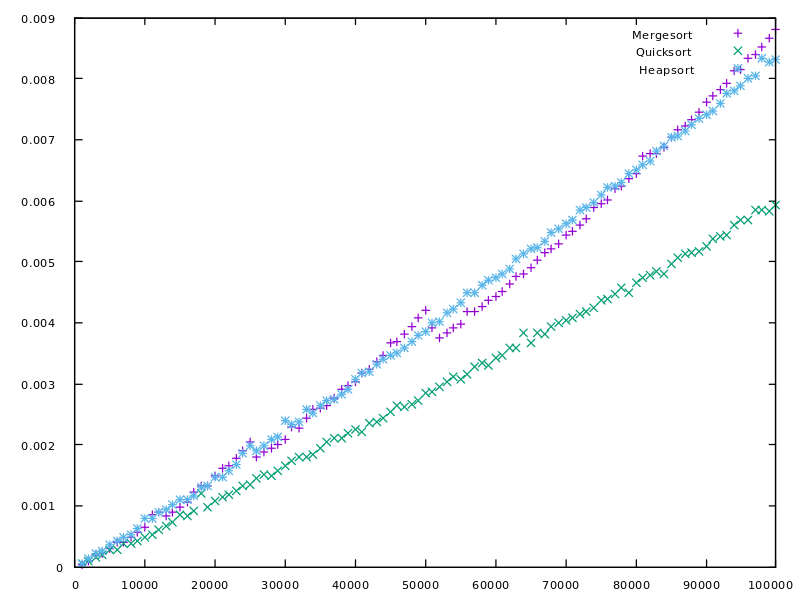
\includegraphics[width=1\textwidth]{nlogn.png}
  \label{fig:ejemplo}
\end{figure}
\end{frame}
\begin{frame}
\frametitle{tablas orden $n^2$}
	\begin{figure}
  \centering
    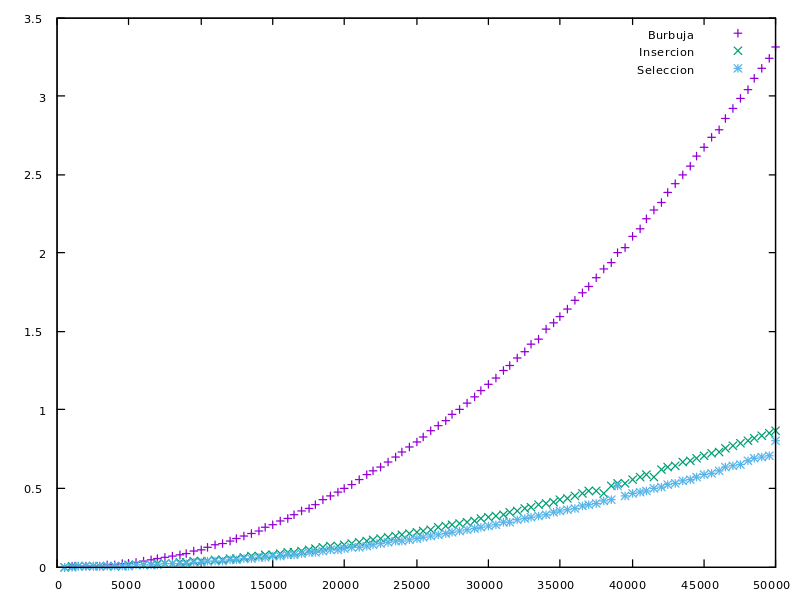
\includegraphics[width=1\textwidth]{Eficiencian2.png}
  \label{fig:ejemplo}
\end{figure}
\end{frame}
\begin{frame}
\frametitle{tablas orden $n^3$}
	\begin{figure}
  \centering
    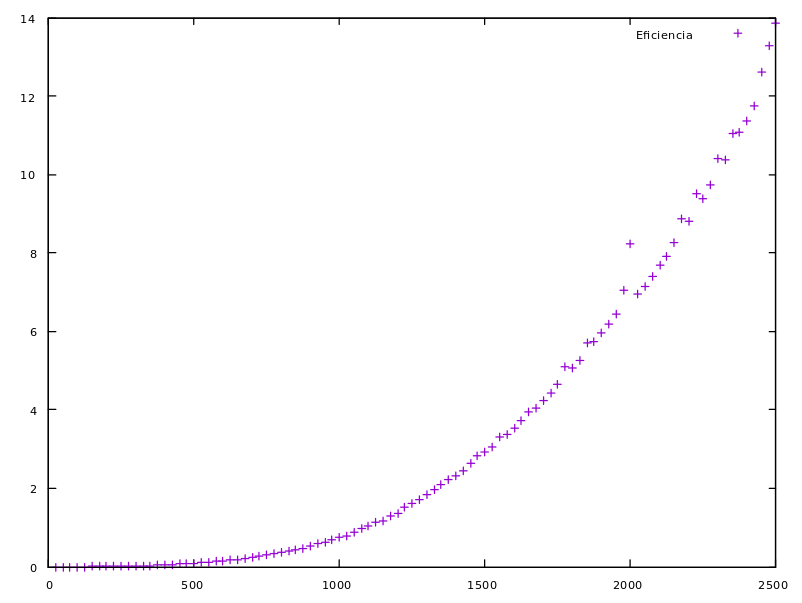
\includegraphics[width=1\textwidth]{Floyd.png}
  \label{fig:ejemplo}
\end{figure}
\end{frame}
\begin{frame}
\frametitle{tablas orden $2^n$}
	\begin{figure}
  \centering
    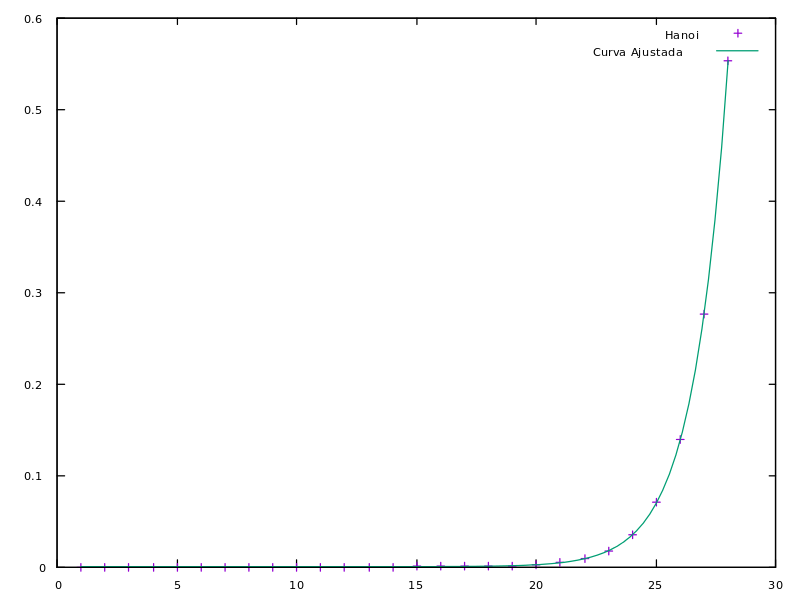
\includegraphics[width=0.98\textwidth]{HanoiAjustada.png}
  \label{fig:ejemplo}
\end{figure}
\end{frame}

\section{Ejercicio 2}
\subsection{enunciado}

\begin{frame}
	2. Con cada una de las tablas anteriores, genere un gráfico comparando los tiempos  de
los algoritmos. Indique claramente el significado de cada serie. Para los algoritmos que
realizan la misma tarea (ordenar) exponga una tabla compartida dondea poder apreciar las diferencias en rendimiento de algoritmos con diferente orden de
eficiencia.
	\begin{figure}
  \centering
    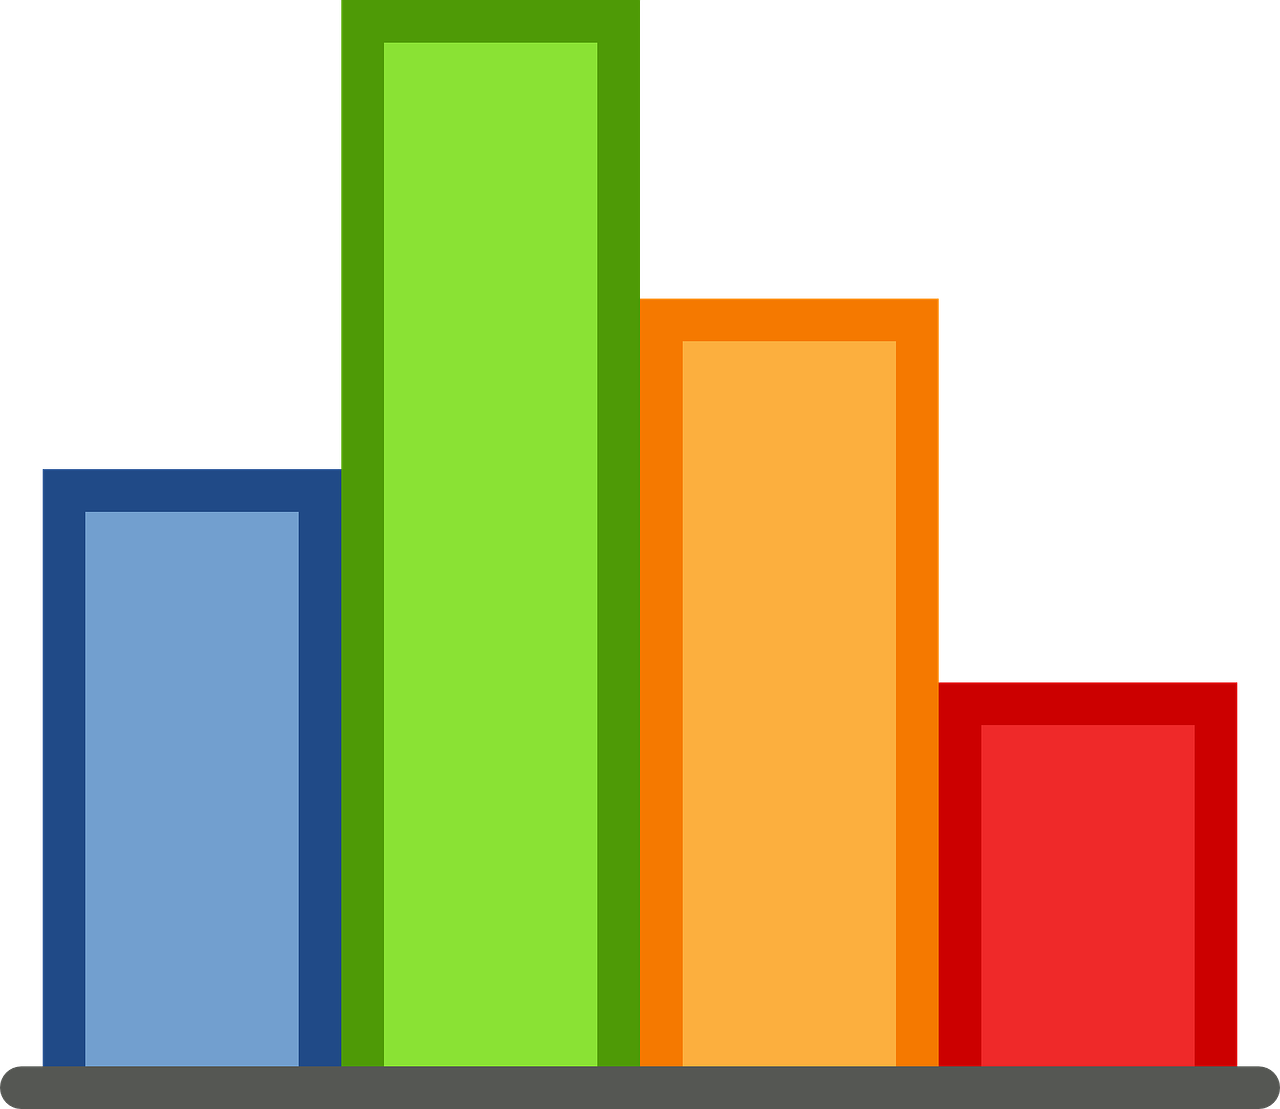
\includegraphics[width=0.3\textwidth]{graf.png}
  \label{fig:ejemplo}
\end{figure}
\end{frame}
\subsection{solución}
\begin{frame}
Las gráficas por ordenes de eficiencia ya las mostramos en el ejercicio anterior. Ahora proseguiremos explicando como las generamos y exponiedo como las hallamos (uso de gnuplot)
\end{frame}
\begin{frame}
\frametitle{Comparación algoritmos ordenación}
	\begin{figure}
  \centering
    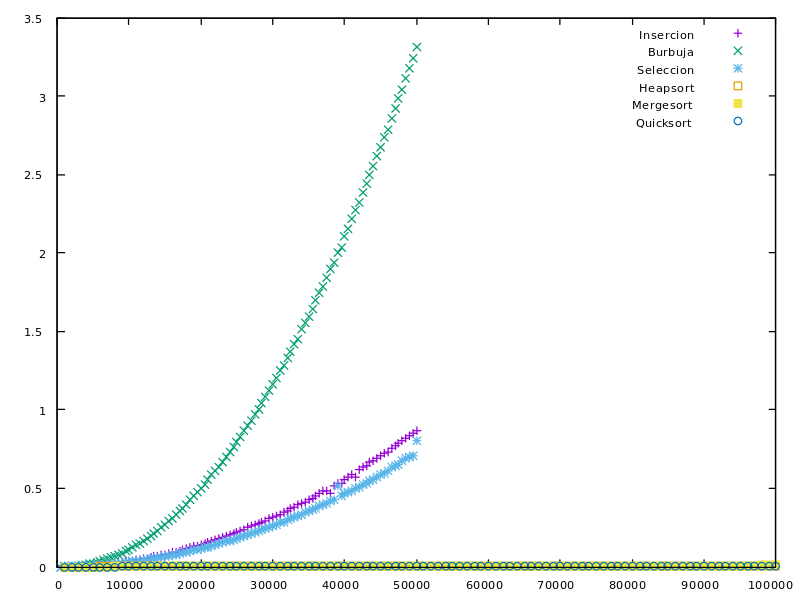
\includegraphics[width=0.98\textwidth]{Ordenacion.png}
  \label{fig:ejemplo}
\end{figure}
	
\end{frame}
\end{document}
